%! Author = Len Washington III
%! Date = 8/12/2023

% Preamble
\documentclass[4]{cs430lecture}

% Packages


% Document
\begin{document}
%<*Lecture-Activity-4>
\maketitle
\newcommand{\sectiontype}{\section}
\begin{enumerate}[label=\arabic*.]
    \item A recurrence relation describes runtime function recursively for a recursive algorithm. Write a recurrence relation for the Merge sort algorithm. HINT: try to count the number of executions of each statement and the cost of each \answer{Recurrence relations for \hyperref[alg:merge-sort]{merge sort} lines: $2=c_{1},3=c_{2},4=5=T\left( \frac{n}{2} \right)$ and $O(n)$ as the runtime for merge\begin{equation*}
			\begin{aligned}
				T(n)&=c_{1}+c_{2}+T\left( \frac{n}{2} \right)+T\left( \frac{n}{2} \right)+O(n)\\
				T(n)&=2T\left( \frac{n}{2} \right)+O(n)\\
			\end{aligned}
			\end{equation*}}
\end{enumerate}

\sectiontype{Solving Recurrence Relations -- Recurrence Tree Method}\label{sec:solving-recurrence-relations-recurrence-tree-method}
\noindent We solve a recurrence relation to get a function in its closed (non-recursive) form. The recurrence tree method is a visual method of repeatedly substituting in the recurrence relation for $T(n)$ on smaller and smaller $n$ until you reach the base case, and then summing up all the nodes in the tree.

\begin{enumerate}[label=\arabic*., start=2]
    \item Draw the recurrence tree for Mergesort \answer{$T(n)=2T\left( \frac{n}{2} \right)+\theta(n)$, $T(1)=O(1)$}\\
	\globaltikzset
	\tikzset{level distance=2.5cm, minimum width=2em}
			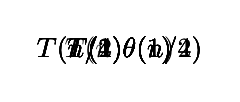
\begin{tikzpicture}
			\Tree
			[.\node{ \sout{$T(n)$}$\theta(n)$ };
				[.\node{ \sout{$T(n/2)$}$\theta(n/2)$ };
					[.\node{ \sout{$T(n/4)$}$\theta(n/4)$ };
						\edge[dashed];\node{ \sout{$T(1)$}$\theta(1)$ };
						\edge[dashed];\node{ \sout{$T(1)$}$\theta(1)$ };
					]
					[.\node{ \sout{$T(n/4)$}$\theta(n/4)$ };
						\edge[dashed];\node{ \sout{$T(1)$}$\theta(1)$ };
						\edge[dashed];\node{ \sout{$T(1)$}$\theta(1)$ };
					]
				]
				[.\node{ \sout{$T(n/2)$}$\theta(n/2)$ };
					[.\node{ \sout{$T(n/4)$}$\theta(n/4)$ };
						\edge[dashed];\node{ \sout{$T(1)$}$\theta(1)$ };
						\edge[dashed];\node{ \sout{$T(1)$}$\theta(1)$ };
					]
					[.\node{ \sout{$T(n/4)$}$\theta(n/4)$ };
						\edge[dashed];\node{ \sout{$T(1)$}$\theta(1)$ };
						\edge[dashed];\node{ \sout{$T(1)$}$\theta(1)$ };
					]
				]
			]
			\end{tikzpicture}
\end{enumerate}

\sectiontype{Divide and Conquer Algorithms}\label{divide-and-conquer}
\begin{itemize}
    \item Divide -- divide the problem into sub-problems that can be solved independently
    \item Conquer -- recursively solve each sub-problem
    \item Combine -- possibly necessary, combine solutions into sub-problems
\end{itemize}
Not all problems can be solved with the divide and conquer approach. Maybe sub-problems are not independent, or solutions to sub-problems cannot be combined to find solution to main problem.

\begin{enumerate}[label=\arabic*.,start=3]
    \item Write a recursive algorithm for Binary Search. Write and solve its recurrence relation.\answer{Divide \& Conquer \& Combine Runtime analysis: \begin{algorithm}[H]
    		\caption{Binary Search Algorithm}\label{alg:binary-search}
    		\begin{algorithmic}[1]
    		\Function{BS}{$A$,key,$i$,$j$}\Comment{Initial call: \Call{BS}{($A$ (sorted), $key$, 1, $n$)}}
				\If{i $\leq$ j}\Comment{Handle Base case not found}
	    			\State k $\gets$ $\lfloor \frac{i+j}{2} \rfloor$
					\If{A[k] == key}
						\State \Return key
					\EndIf
				\EndIf
    		\EndFunction
    		\end{algorithmic} % TODO: Get the rest of this algorithm
    	\end{algorithm}\begin{equation*}
    \begin{aligned}
    	T(n)=O(1)+T\left( \frac{n}{2} \right)\\
    	T(1)=O(1)\\
    \end{aligned}
    \end{equation*}}
    \item Write a recursive algorithm for Selection Sort (or insertion sort or bubble sort). Write and solve its recurrence relation. \begin{algorithm}[H]
    		\caption{Selection Sort Algorithm}\label{alg:selection-sort}
    		\begin{algorithmic}[1]
    		\Function{Select}{$A,i,j$}\Comment{Not a stable sorting algorithm. Initial call: Select(A, 1, n)}
				\If{i $<$ j}\Comment{Base case, 1 item is sorted.}
					% \State k $\gets$ the index of the min item in A from i to j.
					\State minSoFar = A[i]
					\State kk=i
					\For{k=i+1; k$\leq$j; k++}	% TODO: Make sure for looks good
						\If{A[k] $<$ minSoFar}
							\State minSoFar $\gets$ A[k]
							\State kk $\gets$ k
						\EndIf
					\EndFor
					\State Swap A[i] with A[k]
					\State Select(A, i+1, j)
				\EndIf
    		\EndFunction
    		\end{algorithmic}
    	\end{algorithm}\answer{Runtime analysis: $T(n)=T(n-1)+O(n)$, $T(1)=O(1)$}
    \item Describe an efficient divide and conquer algorithm to count the number of times a character appears in a string of length $n$.\begin{algorithm}[H]
    		\caption{Count of char in string}\label{alg:str-count}
    		\begin{algorithmic}[1]
    		\Function{Find\_Count}{S, from, to, char}
    			\If{from $<$ to}
					\State mid $\gets$ (from+to)/2
					\State x $\gets$ Find\_Count(A, from, mid, char)
					\State y $\gets$ Find\_Count(A, mid+1, to, char)
					\State \Return x + y
    			\Else\Comment{1 character left}
					\If{S[from]==char}
						\Return 1
					\Else
						\Return 0
					\EndIf
    			\EndIf
    		\EndFunction
    		\end{algorithmic}
    	\end{algorithm}
\end{enumerate}

\sectiontype{Inductive Proofs} (needed in next lecture to prove a solution to a recurrence relation)
\begin{enumerate}[label=\arabic*),start=6]
    \item What are the three steps in an inductive proof?
	\begin{itemize}
		\item Prove for base case
		\item Assume true for $n$, prove for larger $n$
	\end{itemize}
    \item Use an inductive proof to show the sum of the first $n$ integers is $\frac{n(n+1)}{2}$\answer{\begin{equation*}
    \begin{aligned}
    	\sum_{k=1}^{n}k&=\frac{n(n+1)}{2}\\
    	\sum_{k=1}^{1}k=1&=\frac{1(1+1)}{2}\\
					   1&=\frac{1(2)}{2}\\
					   1&=1
    	\sum_{k=1}^{m}k&=\frac{m(m+1)}{2}\\
    	\sum_{k=1}^{m+1}k&=\frac{(m+1)(m+2)}{2}\\
    	\sum_{k=1}^{m}k+\sum_{m+1}^{m+1} &=\frac{(m)(m+1)}{2}+(m+1)\\
    									 &=\frac{(m)(m+1)}{2}+(m+1)\\
    \end{aligned}
    \end{equation*}}
\end{enumerate}
%</Lecture-Activity-4>

\end{document}